\documentclass[10pt]{article}
%small margins
%\usepackage[margin=1in]{geometry}

%basic math stuff
\usepackage{amsmath, amssymb, amsthm}
\usepackage{mathrsfs, mathtools}
\usepackage{hyperref}
\usepackage[capitalize, noabbrev]{cleveref}
\usepackage{xfrac}
\usepackage{tikz-cd}
\usepackage{float}
\usepackage{enumitem}
\usepackage{mleftright}
\usepackage{cancel} 

%ok
\usepackage{xcolor}
\definecolor{meangreen}{RGB}{0,133,62}
\definecolor{burntorange}{RGB}{191,87,0}

%table of contents formatting
\usepackage{tocloft}
\renewcommand{\cftsecfont}{\color{black}}
\renewcommand{\cftsubsecfont}{\color{burntorange}}
\usepackage{titlesec}

%microtype, font, color support, cl
\usepackage[activate={true,nocompatibility},final,tracking=true,kerning=true,spacing=true,factor=1100,stretch=10,shrink=10]{microtype}
\usepackage{adforn}
%\usepackage[charter]{mathdesign}
%\usepackage[cmintegrals,cmbraces]{newtxmath}
%\usepackage{ebgaramond-maths}
\usepackage[T1]{fontenc}


\usepackage{fancyhdr}
\fancyhf{}
 \fancyhead[RO,LE]{\small\thepage}
 \fancyhead[LO]{\small\itshape\nouppercase{\leftmark}}
 \fancyhead[RE]{\small\itshape Lecture Notes}
 \setlength{\headheight}{11.0pt}
\pagestyle{fancy}

%figures
\usepackage{import}
\usepackage{xifthen}
\usepackage{pdfpages}
\usepackage{transparent}
\newcommand{\incfig}[2][1]{%
    \def\svgwidth{#1\columnwidth}
    \import{./figures/}{#2.pdf_tex}
}
\pdfsuppresswarningpagegroup=1

%good stuff
\newtheorem{theorem}{Theorem}[section]
\newtheorem{lemma}{Lemma}[section]
\newtheorem{cor}{Corollary}[section]
\newtheorem{problem}{Problem}
\newtheorem{prop}{Proposition}[section]
\newtheorem*{prob}{Problem}
\theoremstyle{definition}
\newtheorem*{note}{Note}
\newtheorem*{claim}{Claim}
\newtheorem{definition}{Definition}[section]
\newtheorem{remark}{Remark}[section]
\newtheorem{example}{Example}[section]
\newenvironment{solution}
  {\renewcommand\qedsymbol{$\blacksquare$}\begin{proof}[Solution]}
  {\end{proof}}

%named theorems!
\swapnumbers
\theoremstyle{plain}
\newcommand{\thistheoremname}{}
%numbered
\newtheorem{genericthm}[theorem]{\thistheoremname}
\newenvironment{namedthmnum}[1]
  {\renewcommand{\thistheoremname}{#1}%
         \begin{genericthm}}
        {\end{genericthm}}
%unnumbered
\newtheorem*{genericthm*}{\thistheoremname}
\newenvironment{namedthm}[1]
  {\renewcommand{\thistheoremname}{#1}%
         \begin{genericthm*}}
               {\end{genericthm*}}
%general thing (definition, example, etc)
\theoremstyle{definition}
\newcommand{\thisthingname}{}
\newtheorem{genericthing}[definition]{\thisthingname}
\newenvironment{namedthingnum}[1]
  {\renewcommand{\thisthingname}{#1}%
         \begin{genericthing}}
        {\end{genericthing}}
%unnumbered thing
\newtheorem*{genericthing*}{\thisthingname}
\newenvironment{namedthing}[1]
  {\renewcommand{\thisthingname}{#1}%
         \begin{genericthing*}}
               {\end{genericthing*}}

%self explanatory
\newcommand\N{\ensuremath{\mathbb{N}}} 
\newcommand\R{\ensuremath{\mathbb{R}}} 
\newcommand\A{\ensuremath{\mathbb{A}}} %affine space
\newcommand\Z{\ensuremath{\mathbb{Z}}} 
\renewcommand\O{\ensuremath{\emptyset}} 
\newcommand\Q{\ensuremath{\mathbb{Q}}} 
\newcommand\C{\ensuremath{\mathbb{C}}}
\newcommand\F{\ensuremath{\mathbb{F}}} %field
\newcommand\E{\ensuremath{\mathbb{E}}} %field extension
\renewcommand\P{\ensuremath{\mathbb{P}}} %projective space
\renewcommand\H{\ensuremath{\mathbb{H}}} %hyperbolic space
\newcommand\im{\ensuremath{\operatorname{im}}} %image
\newcommand\id{\ensuremath{\operatorname{id}}} %identity map
\newcommand\grad{\ensuremath{\operatorname{grad}}} %gradient
\newcommand\curl{\ensuremath{\operatorname{curl}}} %gurl
\renewcommand\div{\ensuremath{\operatorname{div}}} %divergence
\newcommand\Gr{\ensuremath{\operatorname{Gr}}} %grassmannian
\newcommand\Hom{\ensuremath{\operatorname{Hom}}} %linear mappings
\newcommand\tr{\ensuremath{\operatorname{tr}}} %trace
\newcommand\supp{\ensuremath{\operatorname{supp}}} %support

\newcommand{\transv}{\mathrel{\text{\tpitchfork}}}
\makeatletter
\newcommand{\tpitchfork}{%
      \vbox{
              \baselineskip\z@skip
                  \lineskip-.52ex
                      \lineskiplimit\maxdimen
                          \m@th
                              \ialign{##\crcr\hidewidth\smash{$-$}\hidewidth\crcr$\pitchfork$\crcr}
                                }%
                            }
                            \makeatother
%transversality

%essential (thanks Dr. Urbanski)
\renewcommand\qedsymbol{$\boxtimes$}

%link colors
\hypersetup{
 linktocpage,
 colorlinks,
 linkcolor={burntorange},
 citecolor={meangreen},
 urlcolor={blue!80!black}
}

%cool section divider
\newcommand{\orbreak}{
\begin{center}
    \adforn{25}\adforn{14}\adforn{53}
 \vspace{0.2cm}
\end{center}
}

%\titleformat{\section}[frame]
%{\normalfont}
%{\filright
%\footnotesize
%\enspace Lecture \thesection\enspace}
%{8pt}
%{\Large\bfseries\filcenter}

  \titlespacing*{\section}
{0pt}{5.5ex plus 1ex minus .2ex}{4.3ex plus .2ex}

%tis me
\author{Simon Xiang}

\title{An Overview of Hyperbolic Manifolds}
\begin{document}
\maketitle
A reading project for the Spring 2021 graduate section of Riemannian Geometry (Math 392C) at UT Austin, taught by Dr.\ Sadun. 
Here, a ``typical reader'' is someone that has just finished this course and knows the basics of covering space theory.
This writeup gives a brief overview of various topics in hyperbolic geometry, concluding with the definition of Teichm\"uller space. Source files: \url{https://git.simonxiang.xyz/math_notes/files.html}

\tableofcontents
\newpage
    \section{Hyperbolic space} 
\subsection{M\"obius transformations}
A \textbf{M\"obius transformation} in $S^n $ is defined as a composition of reflection of $(n-1)$-spheres in $S^n $ that preserve orientation. We call similar transformations that reverse orientation \textbf{anti-M\"obius transformations}. In two dimensions, these are the familiar maps \[
    z \mapsto A(z)= \frac{az+b}{cz+d}, \quad \text{where} \ A=
    \begin{pmatrix}
        a & b \\ c & d
    \end{pmatrix},\ \det A\neq 0.
\] A \textbf{normalized} M\"obius transformation has $\det A=1$; from now we assume M\"obius transformations are normalized. So the group of M\"obius transformations is $\mathrm{PSL}(2,\C)$, as we have seen in class. Two M\"obius transformations $A,B$ are \textbf{conjugate} there exists $U$ another M\"obius transformation such that $B=UAU^{-1}$, and if $A(z)=z$, then $z$ is a \textbf{fixed point} of $A$. If $x_0$ is a fixed point of $A$, then $x_0$ is an \textbf{attracting fixed point} if the function sequence $x, f(x),f(f(x)),f(f(f(x))),\cdots $ converges to $x_0$ for any $x$ in a neighborhood of $x_0$. It can be shown that this is equivalent to saying $|A'(x_0)|<1$, and so \textbf{repelling fixed points} satisfy $|A'(x_0)|>1$, while \textbf{neutral fixed points} satisfy $|A'(x_0)=1|$. We say $A$ is \textbf{parabolic} if either
\begin{itemize}
\setlength\itemsep{-.2em}
    \item $A$ is conjugate to $z \mapsto z+1$,
    \item $\tr A=\pm 2$, $A\neq \id$.
    \item $A$ has exactly one fixed point.
\end{itemize}These conditions are equivalent. Similarly, $A$ is \textbf{elliptic} if 
\begin{itemize}
\setlength\itemsep{-.2em}
    \item $A$ is conjugate to $z \mapsto e^{2i \theta}z,\ 2\theta\not\equiv 2\pi$,
    \item $\tr A \in (-2,2)$,
    \item $A$ has exactly two neutral fixed points,
\end{itemize} and \textbf{loxodromic} if
\begin{itemize}
\setlength\itemsep{-.2em}
    \item $A$ is conjugate to $z \mapsto \lambda^2 z$ for $|\lambda|>1$,
    \item $\tr A \in \C \setminus [-2,2]$.
    \item $A$ has exactly one repelling and one attracting fixed point.
\end{itemize}A M\"obius transformation conjugate to one of the three classes above will be called a  \textbf{standard form}.

\subsection{Hyperbolic geometry}
Euclid's parallel postulate says that for a line and a point not on it, there exists a unique parallel line containing the other point. If we assume that this is false and consider the possibility of an uncountable number of ``parallel'' lines, we get a new framework of geometry, which is now known as \textbf{hyperbolic geometry}. Here are some features of hyperbolic geometry:
\begin{enumerate}[label=(\roman*)]
    \item The angle sum of a hyperbolic triangle $\Delta$ is $\pi- \text{area} \, \Delta$.
    \item There are no ``similarities'' of hyperbolic space--- scaling figures changes angles and shapes. So all hyperbolic triangles with the same angles are isometric, and the choice of unit length is not arbitrary.
    \item For $0 \leq \theta < \frac{\pi}{n-2}$, there exists a unique regular hyperbolic polygon with vertex angles $\theta$.
    \item The hyperbolic volume of a ball and surface area of the bounding sphere grow at an exponential rate as the hyperbolic radius $\rho$ grows. The ratio of surface area to volume approaches 2 as $\rho \to \infty$.
\end{enumerate}
So intuitively there are more shapes, they are more ``rigid'' in a sense, and we have more space to play with them. Many 2-dimensional surfaces and 3-manifolds are well modeled by hyperbolic geometry; for example, embedding exponentially growing graphs to model data\footnote{Source: \url{https://bjlkeng.github.io/posts/hyperbolic-geometry-and-poincare-embeddings}.}, which plays a role in machine learning.
\begin{figure}[H]
\centering
 
\includegraphics[width=0.5\linewidth]{figures/escher.jpg}
 \caption{Obligatory Escher print.} 
 \label{escher} 
\end{figure}
As review, let us discuss the common models of hyperbolic space, which are subsets of $\R^n $ with an appropiate Riemannian metric. The \textbf{upper half-plane model} is the set $\{z \in \C\mid \operatorname{Im}z >0\} $ with the metric $ds= \frac{|dz|}{\operatorname{Im}z}$. The \textbf{unit disk model} is $\{z \in \C \mid |z|< 1\} $ equipped with the metric $ds= \frac{2|dz|}{1-|z|^2}$.\footnote{These are analogous to the metrics $d^2 = \frac{dx^2+dy^2}{y^2}$ and $ds ^2= \frac{4(du ^2+dv ^2)}{(1-u^2-v^2)^2}$.}  Denote either of these models by $\H^2$, the notation for the \textbf{hyperbolic plane}. These models satisfy
\begin{enumerate}[label=(\roman*)]
%\setlength\itemsep{-.2em}
    \item The metrics are \textbf{infinitesimally Euclidian}, or conformal to the standard Euclidian metric $g_{ij}=\delta _{ij}$.
    \item $\H^2$ is \textbf{complete} in its metric, or every arc that approaches the boundary has infinite length.
    \item The metrics are invariant under M\"obius transformations that are also endomorphisms; these transformations actually make up the full group of orientation preserving isometries of the model.
    \item Hyperbolic lines (geodesics) in the upper half-plane model are semicircles orthogonal to $\R$ and vertical half lines. In the disk model, they're diameters and circular arcs orthogonal to the unit circle.
\end{enumerate}
The \textbf{upper half-space model} $\{(z,t) \mid z \in \C, t>0\} $ with 
\[
ds= \frac{|d \vec x|}{t},\quad |d\vec x|^2 = |dz|^2+dt^2
\] 
and the \textbf{ball model} $\{\vec x \in \R^3 \mid  |\vec x|<1\} $ with $ds= \frac{2|d\vec x|}{1- |\vec x|^2}$ are defined analogously, and satisfy similar properties. The difference is that now geodesics in the upper-half space model are hemispheres orthogonal to $\C$ and vertical Euclidian half-planes, while geodesics in the ball model are spherical caps orthogonal to the boundary $S^2$ and equatorial planes.

\subsection{Fixed surfaces of standard forms}

Let $\partial \H^2= S^1 $ or $\R \cup \{\infty\} $ for the hyperbolic plane, and $\partial \H^3=S^2$ or $\C\cup \{\infty\} $ for hyperbolic space. We can also denote these by $S_{\infty}$ for the \textbf{circle or sphere at infinity}. Isometries of $\H^3$ extend to $\partial \H ^3$ as conformal automorphisms. Standing inside a hyperbolic plane, we would see $S_{\infty}$ as the ``horizon'' of the world, while from the outside $\partial \H^3$ is full of circles corresponding to elements of discrete groups of isometries, or \textbf{outer circles}.

\begin{figure}[H]
\centering
 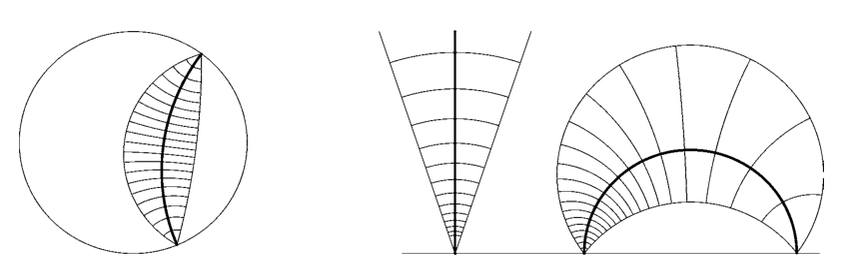
\includegraphics[width=0.7\linewidth]{figures/hyp1.png}
\caption{The fixed axes and surfaces of elliptic and loxodromic transformations.} 
 \label{fix} 
\end{figure}
Elliptic transformations have an \textbf{axis of rotation} in $\H^3$, or the hyperbolic line connecting its fixed points. Loxodromic transformations have a similarly defined axis. Not only do elliptic and loxodromic transformations fix an axis, but they also fix a family of equidistant surfaces from the axis! If the transformation is in standard form, then the surface fixed is a cone with vertex at the origin with the hafl $z$-axis a vertical axis, as in the middle figure of \cref{fix}. If both endpoints lie on the line $t=0$, then the surface fixed is a tube that compresses into a cone as it approaches the boundary points.
\begin{figure}[H]
\centering
 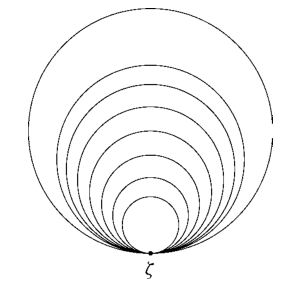
\includegraphics[width=0.3\linewidth]{figures/hyp2.png}
\caption{Horospheres.} 
\label{horo} 
\end{figure}

A parabolic transformation only fixes one point, so no axes are fixed. However, parabolic transformations still have invariant surfaces; they resemble a Euclidian sphere, and are called \textbf{horospheres}.\footnote{Horospheres are not hyperbolic spheres!} A family of horospheres are all tangent to each other and $S_{\infty}$ at a point $\zeta$ as in \cref{horo}, almost like the Hawaiian earring. The region bounded by a horosphere is a \textbf{horoball}: if $\zeta$ is at infinity, then horospheres are Euclidian planes and horoballs are the half-spaces above such planes.

\section{Discrete groups} 
Two groups $G,H$ of M\"obius transformations are \textbf{conjugate} if there exists a M\"obius transformation $T$ such that $G=THT^{-1}$. Note that a torsion-free group of M\"obius transformation has no elliptic elements. For a group $G$ acting on a set $X$, the \textbf{stabilizer} of a subset $\Sigma \subseteq X$ in $G$ is defined as \[
    \operatorname{Stab}_G(\Sigma)= \{g \in G \mid g(\Sigma)=\Sigma\} =\operatorname{Stab}(\Sigma).
\] 
\subsection{Convergence of M\"obius transformations}
\begin{lemma}\label{seq} 
    If $\{T_n \} $ is an infinite sequence of distinct M\"obius transformations such that the corresponding sequences of fixed points $\{p_n \} ,\{q_n \} $\footnote{If the M\"obius transformations $T_n $ are parabolic then $p_n =q_n $. If they're elliptic then the $p_n ,q_n $ are neutral fixed points, and if the $T_n $ are loxodromic then without loss of generality the $p_n $ are repelling while the $q_n $ are attracting.} converge to $p,q \in S^2$, then there is a subsequence $\{T_k\} $ that satisfies one of the following properties:
    \begin{enumerate}[label=(\roman*)]
\item There exists a M\"obius transformation $T$ such that $\lim T_k(z)=T(z)$ uniformly on $\H^3 \cup S^2$ (with the standard Euclidian metric).
\item $\lim T_k(z)=q$ uniformly for all $z\neq p$ on compact subsets of $\H^3 \cup (S^2 \setminus \{p\} )$. Analogously, $\lim T_k ^{-1}(z)=p$ uniformly for all $z\neq q$ on compact subsets of $\H^3 \cup  (S^2 \setminus \{q\} )$.
    \end{enumerate}
\end{lemma}
Note that $p=q$ is a possible case for (ii). The proof has been omitted for brevity.
\begin{cor}
    If $\{T_n \} $ is an infinite sequence of distinct M\"obius transformations and $U \subseteq S^2$ is a connected open set, suppose we have two distinct points $\zeta_1,\zeta_2 \in S ^2$ such that $\zeta_1,\zeta_2 \notin T_n (U)$ for all $n$. Then there exists an infinite subsequence $\{T_m\} $ which converges on $U $ (uniformly on compact subsets) to a M\"obius transformation or a constant.
\end{cor}
This corollary is a stronger form of Montel's theorem from complex analysis.
\begin{lemma}
    If $g$ is loxodromic and $h$ exchanges the fixed points of $g$, then $h^2=\id$, or $\tr h=0$.
\end{lemma}
\begin{proof}
    $h^2$ fixes the fixed points of $g$, which implies that $h^2$ fixes its own fixed point(s).
\end{proof}

\subsection{Discreteness}
If $G$ is a group of M\"obius transformations, then $G$ is \textbf{discrete} if there is no infinite sequence of distinct elements of $G$ converging to the identity of $G$. By \cref{seq}, the following conditions are all equivalent to discreteness:
\begin{enumerate}[label=(\roman*)]
    \item No infinite sequence of distinct elements of $G$ converges to a M\"obius transformation.
    \item The action of $G$ is \textbf{properly discontinuous}; that is, for any closed ball $B \subseteq \H^3$, $\{g \in G\mid g(B)\cap B\neq \O\} $ is finite.
    \item $G$ has no limit points in $\H^3$; that is, for $\vec x \in \H^3$, there is no point $\vec y \in \H^3$ and infinite sequence $\{g_n \} $ in $G$ such that $\lim g_n (\vec y)=\vec x$.
\end{enumerate}
A group $G$ is \textbf{elementary} iff it preserves one point or a pair of points on $S^2$, or a single point in $\H^3$. This is equivalent to saying any two torsion-free elements share a fixed point. 
\begin{namedthm}{J\o{}rgensen's Inequality} 
    If $G=\langle A,B \rangle $ (the group generated by $A,B$) is discrete and non-elementary, then \[
        | \tr ^2 A- 4| + |\tr (ABA^{-1}B^{-1})-2| \geq 1.
    \] If $G$ is elementary, then either 
    \begin{enumerate}[label=(\roman*)]
    \setlength\itemsep{-.2em}
\item $G$ is cyclic/a finite abelian extension of a cyclic group and $|\tr ^2 A-4|<1$,
\item $A$ is loxodromic or elliptic with $|\tr ^2A-4| < \frac{1}{2}$ with $B$ interchanging the fixed points of $A$,
\item $A$ is parabolic while $B$ is parabolic or elliptic of order $2$, $3$, $4$, or $6$ and fixes the fixed point of $A$.
    \end{enumerate}
\end{namedthm}
\begin{cor}
    A non-elementary group $G$ is discrete iff every every two-generator subgroup is discrete. 
\end{cor}

\subsection{Kleinian groups and orbifolds}
\begin{figure}[b]
\centering
 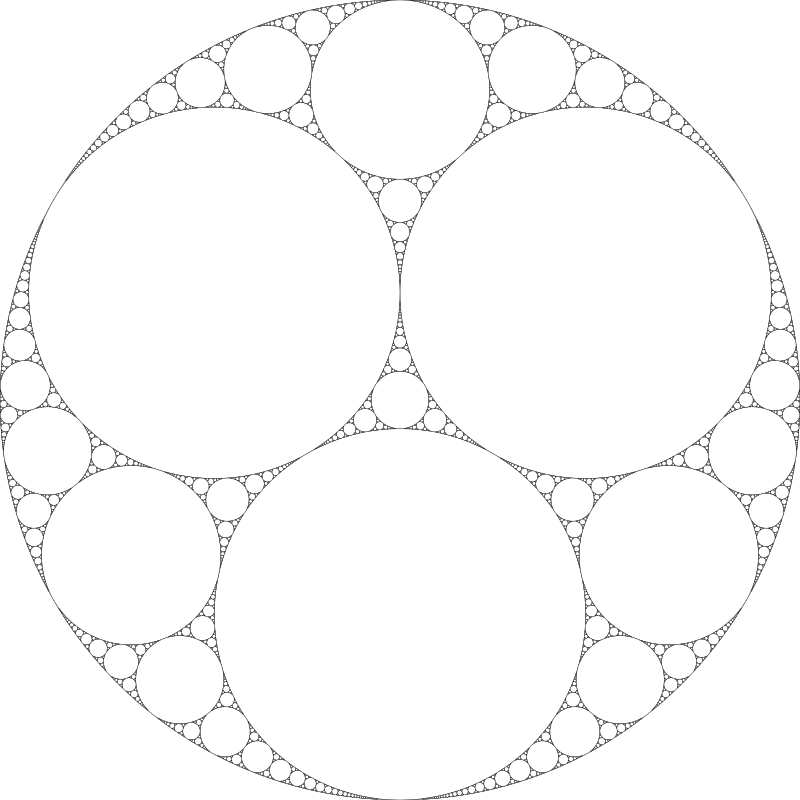
\includegraphics[width=0.4\linewidth]{figures/hyp3.png}
 \caption{An \textit{Apollonian gasket} is a limit set of a Kleinian group.} 
\end{figure}
We say that discrete groups of M\"obius transformations are \textbf{Kleinian groups}, which we assume to be non-elementary. A Kleinian group that preserves the interior of a round disk on $S^2$ is a \textbf{Fuchsian group}. For $\zeta \in S^2$ to be a \textbf{limit point}, there must exist some $\xi \in S^2$ satisfying $\lim T_n (\xi)=\zeta$ for some infinite sequence $\{T_n \} $ where the $T_n \in G$ for all $n$. Define the \textbf{limit set} by \[
    \Lambda(G)= \{\zeta \in S^2\mid \zeta \ \text{is a limit point} \} .
\] It contains all loxodromic and parabolic fixed points and is preserved by $G$, and if $\Lambda(G)$ has less than three points, $G$ is an elementary group. 
Define \[
\Omega(G)= S^2 \setminus \Lambda(G) 
\] to be the \textbf{ordinary set}, which is also preserved under $G$. We study Kleinian groups by considering the quotient space \[
\mathcal{M} (G)=(\H^3 \cup \Omega(G)) / G,\quad \partial \mathcal M(G)= \Omega(G) /G.
\] If $G$ is torsion-free (contains no elliptics), then $\mathcal{M} (G)$ is an oriented manifold with boundary (possibly empty) and the quotient projection $\pi \colon \H^3 \cup  \Omega \to \mathcal{M} $ is a local homeomorphism $\H^3 \to \H^3 / G:= \mathcal{M} (G)^{\text{int}}$, $\Omega \to \Omega(G) /G = \partial \mathcal{M} (G)$. Then $\mathcal{M} (G)^{\text{int}}$ inherits a quotient metric from $\H^3$, and $\pi_1(\mathcal{M} )\approx G$. If $G$ contains elliptics, then $\mathcal{M} (G)$ is an \textbf{orbifold}. 

Although the ``boundary'' $\partial \mathcal{M} (G)$ is very far from any interior point (with respect to the hyperbolic metric) in $\mathcal{M} (G)^{\text{int} }$, it is closely related to the interior structure. Isometries and geodesics extend to the boundary, and the boundary $\partial \mathcal{M} (G)$ has a conformal structure induced by $\Omega(G) \subseteq S^2$. So $\partial \mathcal{M} (G)$ is called the \textbf{conformal boundary} of $\mathcal{M} (G)$.

\begin{namedthm}{Ahlfors Finiteness Theorem} 
    If $G$ is a finitely generated Kleinian group, then $\partial \mathcal{M} (G) = \Omega(G) /G$ is the union of a finite number of surfaces, each of which is a compact Riemann surface with a finite amount of points removed.
\end{namedthm}
A natural question to ask here is ``what is a Riemann surface''?

\section{Riemann surfaces}

Riemann surfaces are complex analytic 1-manifolds.\footnote{Similar to smooth manifolds, \emph{analytic} manifolds have analytic transition maps. Complex manifolds have charts homeomorphic to $\C^n $ as opposed to $\R^n $.} Note that Riemann surfaces are orientable since holomorphic maps preserve orientation. A \textbf{conformal mapping} is a homeomorphism $f \colon R \to S$ between Riemann surfaces such that $\phi_{\beta }f \phi_{\alpha }^{-1}$ is conformal, where $\phi_{\beta },\phi_{\alpha }$ are chart homeomorphisms. 

Riemann surfaces have a ``rule'' (typically from a Riemannian metric) for measuring angles. For example, consider a region $\Omega \subseteq \C$ with Euclidian angles. Define a rule for measuring angles by taking the angle between two rays at a point $z$ and sending it to the resultant angle after applying a transformation $T\colon (x,y) \mapsto (x,2y)$. This determines a new Riemann surface structure $T(\Omega)$ on the underlying set, however $\Omega$ is still conformally equivalent to $T(\Omega)$ with the structure from $\C$.

\begin{figure}[H]
\centering
 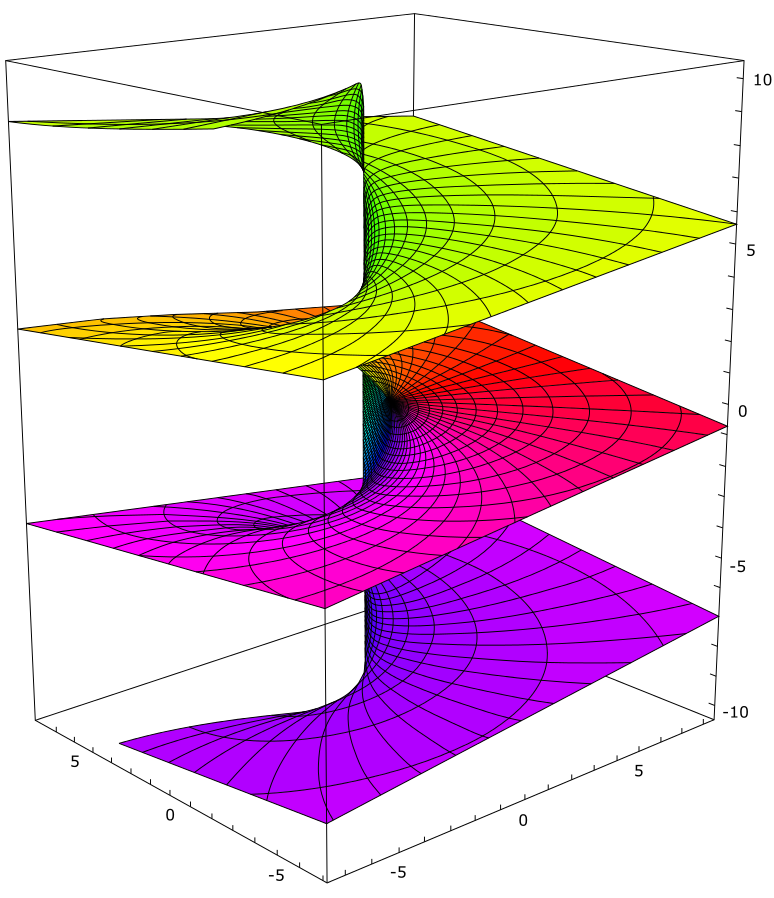
\includegraphics[width=0.4\linewidth]{figures/hyp4.png}
 \caption{The Riemann surface of the complex logarithm.} 
\end{figure}
A covering of a Riemann surface is also a Riemann surface by lifting the local complex structure. On the same vein, deck transformations are just conformal automorphisms of the upstairs cover.

\subsection{Uniformization and Hyperbolization}
If $P(x,y)$ is an irreducible polynomial, then $R= \{(x,y) \in \C^2 \mid P(x,y)=0\} $ is a Riemann surface.\footnote{It actually turns out you can write all Riemann surfaces of this form, by embedding in $\C\mathrm{P}^3$, then applying Chow's theorem, which says any closed holomorphic submanifold of $\C\mathrm{P}^n $ is a smooth algebraic variety. An algebraic variety is just a zero set of polynomials.} An example of such surfaces include zeroes of the \emph{Fermat curves} $x^n+y^n =1,n\geq 2$, representing closed Riemann surface of genus $\frac{1}{2}(n-1)(n-2)$. We would like to find a complex parameter $t$ such that $x=x(t),y=y(t)$ for all $(x,y)=0$.
\begin{namedthm}{Uniformization Theorem} 
    Any simply connected Riemann surface can be conformally mapped to either the Riemann sphere ($S^2$), the complex plane $\C$, or the unit disk $\mathbb D$.  
\end{namedthm}
The third case is just the Riemann mapping theorem. We can apply this to the universal cover $\widetilde R$ of a Riemann surface $R$.
\begin{namedthm}{Uniformization Theorem (for the universal cover)} 
   $\widetilde R$ can be conformally mapped to $S^2$ if $R$ is conformally $S^2$, $\C$ if $R$ is conformally $\C$, $\C\setminus \{0\} $, or a torus, and $\mathbb D$ otherwise. 
\end{namedthm}
If $\Gamma$ denotes the group of deck transformations, then $\Gamma \approx \pi_1(R)$. In this case, deck transformations are conformal automorphisms which are M\"obius transformations in one of the standard models. Deck transformations cannot fix points in the cover, and therefore cannot be elliptic. We also have that $\Gamma$ is properly discontinuous, and so $\Gamma $ is a discrete group. Furthermore, $\Gamma$ is discrete iff  $\pi_1(R)$ is nonabelian.
\begin{namedthm}{Hyperbolization Theorem} 
Every Riemann surface with a nonabelian fundamental group can be equipped with a hyperbolic metric compatible with its complex structure.
\end{namedthm}
Our Uniformization and Hyperbolization theorems tell us that when $\widetilde R=\mathbb D$, we can consider both the complex and hyperbolic structure on $\mathbb D=\H^2$. $\Gamma$ consists of conformal automorphisms, and $\mathbb D$ induces a complex structure on $R = \mathbb D / \Gamma$. Since $\Gamma$ is also a group of isometries of $\H^2$, the hyperbolic structure of $\H^2=\mathbb D$ also induces one on $R=\H^2 / \Gamma$. To explicitly see how, let $z \in \mathbb D$. For $w=\pi(z) \in R$ (the image of $z$ under the covering projection), define the hyperbolic metric on $R$ by \[
    \lambda(w)|dw|=\rho(z)|dz|,
\] where $\rho |dz|$ is the hyperbolic metric on $\mathbb \H^2$. Computing $\lambda$ by $z= \pi ^{-1}(w)$ is usually hard, but we can do this for the punctured disk and the annulus. $R$ has finite hyperbolic area iff it is a closed Riemann surface of nonzero genus $g$ with $n\geq 0$ punctures satisfying $2g+n\geq 3$. The hyperbolic area is $2\pi (2g+n-2)$. For example, consider the punctured sphere with $g=1,$ $n=1$, so the hyperbolic area is $2\pi(2+1-2)=2\pi$.

In $R$ a Riemann surface, we can do analysis (analytic and meromorphic functions, etc) by the complex structure, and geometry (geodesics, area, etc) by the hyperbolic structure. The uniformization/hyperbolization reconciles these ideas by suggesting we do both analysis and geometry in the universal cover $\widetilde R$, keeping in mind the group of deck transformations $\Gamma$.

\subsection{Teichm\"uller spaces of Riemann surfaces}
Consider a smooth nonsingular Riemannian metric \[
ds ^2=E dx^2+2F dx\,dy+G dy^2,
\] which we can rewrite as $ds ^2=\lambda(z)|dz+\mu(z)d \bar{z}|^2$ for $\lambda(z)>0$ and $0 \leq |\mu(z)| <1$. If $\mu=0$, then this is a \textbf{conformal metric} $|dw|=\lambda(z)|dz|$. If we have a Riemannian metric, we can introduce new local coordinates on a surface such that the new metric is conformal--- this process goes by ``introducing \textbf{isothermal coordinates}''. We can introduce isothermal coordinates if 
\begin{equation}\label{bel} 
\frac{\partial F}{\partial \bar z}=\mu(z) \frac{\partial F}{\partial z}.
\end{equation}\cref{bel} is called the \textbf{Beltrami equation}. 
    For example, for the metric $ds ^2=|dz +k d \bar z |^2$ on $\C$, the map $w=F(z)=z+k \bar z,\, z \in \C,\, 0 <k<1$ solves the Beltrami equation with $\mu=k$. This sends circles about $z=0$ to ellipses with major and minor axes in the ratio $K=\frac{1+k}{1-k}$. Solutions to the Beltrami equation are $\mathbf K$\textbf{-quasiconformal mappings}. If $\|\mu\|_{\infty}<1$,\footnote{Here, $\|\mu\|_{\infty}$ refers to the essential supremum of $\mu$.} then a solution, or $K$-quasiconformal mapping, exists.

        Let $R= \H ^2/ G$ be a closed Riemann surface of nonzero genus $g$ and $n\geq 0$ punctures satisfying $3g+n-3>0$. Define the \textbf{Teichm\"uller space} $\operatorname{Tiech}(R)$ as the quotient \[
            \operatorname{Teich}(R) =\{(S,f) \mid f \colon R \to S \ \text{is quasiconformal}\} / \sim,
        \] modulo the equivalence relation $(S,f)\sim (S',f') \ \text{iff} \ f' \circ f^{-1} \colon S \to S'$ is homotopic to a conformal map. For $\alpha  \colon R \to R$ a quasiconformal automorphism, the homotopy class of $\alpha $ determines an automorphism $\alpha $ of $\operatorname{Teich}(R)$ by $\alpha  \colon (S,f) \to (S,f \circ \alpha )$ up to equivalence. Then the homotopy classes $[\alpha ]$ form a group, called the \textbf{mapping class group} (or \emph{Teichm\"uller modular group}) $\mathfrak M(R)$. The mapping class group acts discontinuously on $\operatorname{Teich}(R)$, and the quotient orbifold $\operatorname{Teich}(R) / \mathfrak M(R)$ is the called the \textbf{moduli space}.

\orbreak
Thank you for reading my paper!

\end{document}
